%%%%%%%%%%%%%%%%%%%%%%%%%%%%%%%%%%%%%%%%%%%%%%%%%%%%%%%%%%%%%%%%%%%%%%%%%%%%
%% Trim Size : 11in x 8.5in
%% Text Area : 9.6in (include Runningheads) x 7in
%% ws-jai.tex, 26 April 2012
%% Tex file to use with ws-jai.cls written in Latex2E.
%% The content, structure, format and layout of this style file is the
%% property of World Scientific Publishing Co. Pte. Ltd.
%%%%%%%%%%%%%%%%%%%%%%%%%%%%%%%%%%%%%%%%%%%%%%%%%%%%%%%%%%%%%%%%%%%%%%%%%%%%
%%

%\documentclass[draft]{ws-jai}
\documentclass{ws-jai}
%\usepackage[flushleft]{threeparttable}
%\usepackage{pdflscape}
\usepackage{longtable}
%\usepackage{caption}
\usepackage{subcaption}
%\usepackage{subfig}
\def\btex{B{\sc IB}\TeX\ }
\begin{document}

\catchline{}{}{}{}{} % Publisher's Area please ignore

\markboth{Jack Hickish, CASPER gang, etc.}{The Collaboration for Astronomy
Signal Processing and Electronics Research in 2016.}

\title{The Collaboration for Astronomy Signal Processing and Electronics
Research in 2016}

%\author{First Author$^\dagger$, Second Author$^\ddagger$, Third
%Author$^\ddagger$ and Fourth Author$^\S$}
\author{Jack Hickish$^\dagger$, Others$^\ddagger$}

\address{ $^\dagger$Radio Astronomy Laboratory, UC Berkeley, Berkeley, CA
94720, USA, jackh@astro.berkeley.edu\\ $^\ddagger$Group, Company, Address,
City, State ZIP/Zone, Country\\ $^\S$Group, Company, Address, City, State
ZIP/Zone, Country, fauthor@company.com }

\maketitle

\corres{$^\dagger$Jack Hickish}

\begin{history} \received{(to be inserted by publisher)}; \revised{(to be
inserted by publisher)}; \accepted{(to be inserted by publisher)};
\end{history}

\begin{abstract}

The Collaboration for Astronomy Signal Processing and Electronics Research
(CASPER) has been working for a decade to reduce the time and cost of
designing, building and deploying new digital radio astronomy instruments.
Today, CASPER-designed hardware powers over 40 scientific instruments
worldwide, and are used by scientists and engineers at dozens of academic
institutions.  In this paper we summarize the current offerings of the CASPER
collaboration, focusing on currently-available and next-generation hardware.
We describe the ongoing state of software development, as CASPER looks to
support an ever-increasing selection of off-the-shelf digital signal processing
platforms.

\end{abstract}

\keywords{CASPER, digital signal processing, radio astronomy, instrumentation}

\section{Introduction}

Since the pioneering work of \cite{Weinreb} we
have seen a growing adoption of digital processing hardware as the foundation
on which radio telescopes are built.  Today, CPUs, GPUs, FPGAs and ASICs power
almost all of the world's radio telescopes, and our ability to do science has
become inextricably linked with our ability to perform digital computation.
With the capability of digital processing hardware scaling exponentially with
Moore's law, the ability to leverage current technology by reducing the
design-time of new instruments is critical in effective deployments of new
radio astronomy instruments.

The Collaboration for Astronomy Signal Processing and Electronics Research
(CASPER\footnote{\url{https://casper.berkeley.edu}}) puts
\emph{time-to-science}, the time between conception of an instrument and its
deployment, as a central figure of merit in instrument design. CASPER works to
minimize time-to-science by developing and supporting open-source,
general-purpose hardware, software libraries and programming tools which allow
rapid instrument design, straightforward upgrade cycles and reduced engineering time and cost.

CASPER hardware and software now powers over 40 radio astronomy
instruments worldwide (see Tables~\ref{table:casper-instruments-spectrometers},
\ref{table:casper-instruments-mkids},
\ref{table:casper-instruments-correlators}) including some of the largest, most
advanced telescopes ever built, such as the upcoming MeerKat
Array\footnote{\url{http://public.ska.ac.za/meerkat/meerkat-schedule}}, the
newly commissioned Five-hundred metre Spherical Aperture Telescope (FAST,
\cite{fast}), and the Robert C. Byrd Green Bank Telescope \citep{vegas}. This paper
provides an updaate on the state of the collaboration, which is in the process of releasing
two new FPGA boards to the radio-astronomy community and has recently overhauled
its FPGA-programming toolflow to improve future extensibility and support the latest Xilinx software.

We first summarize the design philosophy of CASPER in
Section~\ref{sec:CASPER-philosophy}.  In Section~\ref{sec:Hardware} we describe
currently available CASPER hardware offerings, including the range of
digitizers developed and supported by CASPER. Key to CASPER's success are the
firmware libraries and programming infrastructure provided by the
collaboration, which we overview in Section~\ref{sec:Software}.  In
Section~\ref{sec:Deployments} we document the extensive and wide-ranging
applications to which CASPER hardware and design-tools have been applied.
Finally, we describe the future direction of and challenges faced by the CASPER
collaboration in Section~\ref{sec:Future}, with concluding remarks in
Section~\ref{sec:Conclusions}.

\section{The CASPER Philosophy} \label{sec:CASPER-philosophy}

%% Jason Manley's PHD has a good section on Philosophy and Ethernet.
The CASPER philosophy is that minimizing time-to-science is a priority when designing instrumentation. CASPER promotes open-source hardware, software and programming tools, which can be collectively developed by the community and re-used in multiple experiments to best leverage the cost and time of development.
The CASPER philosophy advocates keeping the hardware development efforts of an instrument as low as possible, and achieving cost efficiency through regular upgrades, allowing instruments to best exploit Moore's law.

This is in contrast to the way radio telescopes have been built in the past.
Large instruments, for example the ALMA correlator \citep{alma-correlator} and
eVLA's ``WIDAR'' correlator \citep{evla}, have been constructed using
custom-designed Application Specific Integrated Circuits (ASICs) specialised
backplane and cable-based interconnect in an attempt to maximise compute
density, and minimise power and cost. While there are arguments to be made for specialization of systems at this scale, such projects require large
hardware development budgets and timescales, and typically result in complex
and specialised instruments which lag behind the current state-of-the-art when they are deployed and are expensive to upgrade without significant
re-investment of time and money. Moreover, this development effort often does not have a significant impact on the field as a whole, as specialization tends to limit the utility of the designed system for other applications.

In contrast, CASPER's design philosophy allows groups with the expertise and
budgets to develop hardware to benefit the entire community. To this end, the collaboration
is responsible for the development of several generations of open-source FPGA hardware which are compatible with a suite of analog-to-digital converters (ADCs) and digital-to-analog converter (DAC) modules. These boards are accompanied by a suite of open-source parameterized libraries, designed to cater for the wide-ranging needs of the radio astronomy community, and an FPGA-programming toolflow enabling portability of designs between generations of hardware.

\subsection{Modularity}

To a large extent real-time processing tasks in a modern
radio-astronomy instrument can be broken up into commin parts; Namely:
\begin{enumerate}
    \item Digitization of the analog sky signal, which may follow occur after
    some variety of analog down-conversion process. In a multi-receiver telescope, the digitization process can be parellelized over signals from multiple feeds.
    
    \item Channelization of the digitized signal into a discrete number of
    frequency bins, which is accomplished using an FFT-based filterbank
    \citep{specbook}. The channelization proceedure may also be parallelized over signals from different feeds.
    
    \item Combination of signals from multiple antennas either via weighted addition (i.e., beamforming) or via multiplication (i.e.,
    correlation). In either case, it is possible to easily parallelize processing
    over multiple frequency channels.
\end{enumerate}

The details associated with individual instruments vary widely depending
on telescope and application. For example, some telescopes may implement
their channelizers in multiple stages, or may require overlapping filterbanks. Arrays may have widely varying numbers and configurations of antennas and may require correlators with features such as fringe-stopping and delay-tracking.
However, the recognition that
processing can effectively be divided into modular units, some processing data
from only certain antennas (in the case of digitization and channelization) and
some processing data from only certain frequency channels (as is the case for
correlation and beamforming) opens up the opportunity to utilize
general-purpose computing modules, replicated as needed to meet the computation
requirements of the instrument at hand. Where the parallelization changes from
per-antenna to per-frequency, a flexible industry-standard interconnect
solution such as Ethernet can be used to intelligently manage the
data transpose (usually refered to as the \emph{corner turn}) between
per-antenna and per-channel processors.

This is the architecture that underpins the CASPER philosophy: simple,
general-purpose compute modules, with industry-standard commercial
interconnect. Such a modular architecture makes it straightforward to upgrade hardware
piecemeal as Moore's law drives increases in computational capacity of
individual modules. Flexibility of modules increases the ability of multiple
groups to share hardware, and minimises overall cost of design and manufacture.

The use of Ethernet for interconnect makes it simple for instruments to be
constructed which consist of different types of data processing hardware. For example, it is possible
to utilise FPGA technology for applications where IO-rates are critical, such
as when interfacing with digitizers, while handing off other computationally
dense parts of the processing chain to GPU clusters. A
design can even leverage the IP Multicast protocol
%\footnote{IP multicast is described in RFC 1112}
which allows compute nodes to subscribe to
specific data streams and process them concurrently alongside other instruments (Figure~\ref{fig:ethernet-instrument}).
%This keeps the
%problem of full cross-bar interconnects in the domain of the switch
%manufactures and allows instrument designers to focus on digital signal
%processing \citep{man14, pars05}.
Though CASPER has championed the use of multicast switches for many years, only recently has the ability to run multiple instruments simultaneously using multicast to duplicate data streams been demonstrated in an astronomy setting \citep{man14}. 

\begin{figure}
 \centering
 \includegraphics[width=0.7\textwidth]{./ethernet-instrument.pdf}
 % ethernet-instrument.pdf: 792x612 pixel, 72dpi, 27.94x21.59 cm, bb=0 0 792 612
 \caption{The canonical CASPER architecture. $N$ antennas are digitized and channelized into $M$ sub-bands using $N$ processors. These sub-bands are processed by $L$ correlation or beamforming nodes. Other users can subscribe to data streams and simultaneously implement, for example, high-resolution spectrometers or other features.}
 \label{fig:ethernet-instrument}
\end{figure}



%
%
%World-wide, the radio astronomy community is realtively small and has minimal
%financial incentive attracting investors. This means that often institutions
%often rely heavily on government funding. It is therefore beneficial to share
%resources between organisations as to leverage the work that others have put
%into developing radio astronomy instrumentation. For this reason institutions
%often open source their intellectual property. CASPER was founded to aid this
%collaboration. It aims to share and collaborate on both hardware and software
%for the design of radio astronomy DSP systems.
%
%The CASPER community has designed multiple FPGA based hardware platforms and
%the software tools to design and support these platforms.
%

\subsection{Flexibility}

The maximum benefits of modular hardware elements can only be obtained with similarly flexible software and firmware libraries and programming tools that make it simple to put hardware to use and easily upgrade between different hardware generations. Along with hardware platforms, CASPER provides a tool-flow with an interface built on Matlab, Simulink and Xilinx System Generator (XSG) which enables a designer to easily
design and target their chosen hardware platform \cite{pars05}. The interface, described in more detail in Section~\ref{toolflow}, 
is a graphical design environment where a designer can drag and
drop computational blocks from a provided library and connect them with wires in the desired configuration.
The toolflow and library elements are designed to be intuitive to use and provides a ``One-Click'' solution from design to
bitstream, ready to upload onto a board. The flow is designed to reduce the knowledge barrier to entry and allow students and researchers unfamiliar with FPGA technology to rapidly build their own instruments.

\subsection{Community}
The CASPER collaboration currently has over 500 subscribers to its maillist, where users and developers share knowledge, instrument designs and troubleshooting advice. CASPER holds a yearly workshop usually with around 100 attendees, where users and developers may present their instrumentation work, as well as attend tutorial sessions. Groups thinking of deploying instruments based on CASPER hardware are keenly encouraged to visit experienced users who work at various academic institutions worldwide.
The collaboration places a particular emphasis on encouraging students--particularly those who may lack formal training in DSP and FPGA design--to take on instrument design projects.

The collaboration also endeavours to maintain strong links with non-CASPER instrumentation groups, in order to minimize duplication of development efforts. 

\subsection{Design re-use}
The \emph{time-to-science} metric is influenced by the ability to
reuse designs. Just as in the world of software reuse, reuse of
firmware and instrument designs is critical to time-to-science. The
first use of CASPER in a common-user instrument (to my knowledge... -
JMF) was in the Green Bank Ultimate Pulsar Processing
Instrument~\cite{guppi}, which used the gateware libraries
developed by the CASPER group during its inital NSF funded phase.
These libraries were combined with custom firmware blocks and software
to form GUPPI, a very successful instrument to this day.  GUPPI was
built in only about 18 months from the start of the project until
first light observations were recorded.  The machine's hardware
consists of exclusively off-the-shelf CASPER hardware and commodity
computer systems.  In addition to the ease of building the instrument
in the first place, there have been two exact copies made of the
system.  One copy was used locally in Green Bank to process signals
from the retired 140 ft telescope, and a second copy was installed as
the primary pulsar machine at the Arecibo Observatory.  Both of these
machines were installed with no engineering effort, and a modest
effort from the computer system administrators and pulsar scientists.
\emph{In the past, these clonings would have been much more time and
  labor-intensive, hence more expensive.}

The next generation of designs to be created in Green Bank from CASPER
were all based on the ROACH family of configurable signal processors.
As noted in Table~\ref{table:casper-instruments-spectrometers}, several ROACH-1 based spectrometers
are deployed in Green Bank performing various functions for PI based
science~\cite{gbtrans, skynet}.  These all use common
hardware and firmware, and a great deal of the software for processing
and analyzing the output is common as well.  None of the PI based
science would have been feasible without the ease of reuse of the
ROACH designs.

In 2013(?), the NSF funded an effort by UC Berkeley in conjunction
with Green Bank to design the next generation spectrometer for the
GBT.  The new spectrometer was designed to process the data from the
small focal plane array receivers being constructed for the GBT, namely
the 7 pixel (dual-pol) K-band receiver, and a 16 pixel (single-pol)
W-band receiver.  The resulting VEGAS
spectrometer~\cite{chennamangalam2014gpu} was built with reused GUPPI
software, reused CASPER gateware libraries, and new custom gateware
blocks that were subsequently added to the CASPER libraries for others
to use.  Calibration algorithms for the ADCs was gleaned from other
CASPER users~\cite{Jack and Rurik}.  Hardware for interfacing the
spectrometer to the telescope was designed by NRAO and is available to
the community.  The entire VEGAS spectrometer has been cloned and
enhanced as well, and has been deployed at telescopes in China as well
as in other spectrometers in Green Bank.  The enhancements from these
other deployments were then retrofitted to the original VEGAS system,
enhancing its abilities.

Meanwhile, a frequency-multiplexing system for reading out kinetinc
inductance detectors was produced using the ROACH systems for the
ARCONS project.  This system was adapted for the MUSTANG project which
provided a large-format bolometer array detector for the GBT.  The
ARCONS firmware was modified and repurposed for MUSTANG using the same
hardware platforms. 

Others?  EHT? VLBI?

Design reuse has been a driving force behind the CASPER collaboration.
Hardware, software, and firmware reuse all play into the theme of
reducing \emph{time-to-science}.  As a happy coincidence, reducing
time-to-science also reduces cost in many cases.

\section{CASPER Hardware} \label{sec:Hardware}

While CASPER advocates the use of a variety of hardware platforms over the past decade the collaboration has focussed its efforts on designing FPGA-based hardware and ADC/DAC daughterboards\footnote{See \url{https://casper.berkeley.edu/wiki/Hardware}}. Originally utilising processing hardware developed at the Berkeley Wireless Research Center such as the Interconnect Break-out Board (iBOB) and Berkeley Emulation Engine 2 (BEE2, \cite{bee2}) the collaboration later began designing their own platforms to best meet the needs of the radio astronomy community. An overview of the harware specs of the most recent five CASPER boards is given in Table~\ref{table:fpga-hardware}. A dozen different ADC and DAC add-on cards are available for these platforms (Table~\ref{table:adc-hardware}). A brief overview of available FPGA platforms, focussing on the latest-generation SKARAB and SNAP boards, is given below.

\begin{table}
\label{table:fpga-hardware}
\caption{A decade of CASPER hardware.}
\centering
\begin{tabular}{lccccc}
 & iBoB & ROACH & ROACH2 & SNAP & SKARAB \\
\hline
Year Available    & 2005     & 2009     & 2010        & 2016        & 2016               \\
Logic cells       & 53K      & 94K      & 476K        & 162-406K    & 693K               \\
DSP slices        & 232      & 640      & 2016        & 600-1540    & 3600               \\
BRAM capacity     & 4.2 Mb   & 8.8 Mb   & 38 Mb       & 11-28 Mb    & 53 Mb              \\
SRAM capacity     & 2x18 Mb  & 2x36 Mb  & 4x144 Mb    & -           & -                  \\
SRAM bandwidth    & 9 Gb/s   & 43 Gb/s  & 200 Gb/s    & -           & -                  \\
DDR capacity (max)& -        & 1x8 Gb   & 1x16 Gb     & -           & -                  \\
DDR bandwidth     & -        & 38 Gb/s  & 50 Gb/s     & -           & -                  \\
HMC capacity      & -        & -        &             & -           & $<$8x32 Gb         \\
HMC bandwidth     & -        & -        &             & -           & $<$8x30 Gb/s       \\
Ethernet ports    & 2x10 GbE & 4x10 GbE & 8x10 GbE    & 2x10 GbE    & $<$16x40 GbE       \\
ADC/DAC support   & 2xZDOK   & 2xZDOK   & 2xZDOK      & 1xZDOK, 3xHMCAD1511 & 4xMegarray \\
\end{tabular}
\end{table}

\begin{table}
\label{table:adc-hardware}
\caption{CASPER ADC and DAC boards developed for use with FPGA-platforms.}
\centering
\begin{tabular}{lccccc}
Name & Type & Bits & Sample Rate & Inputs/Outputs & Interface \\
\hline
ADC2x1000-8 (iADC) & ADC & 8  & 1 GSPS   & 2 & Z-DOK \\
ADC1x3000-8        & ADC & 8  & 3 GSPS   & 1 & Z-DOK \\
ADC64x64-12        & ADC & 12 & 64 MSPS  & 64 & Z-DOK x2 \\
ADC4x250-8 (QuADC) & ADC & 8  & 250 MSPS & 4 & Z-DOK \\
ADC2x550-12        & ADC & 12 & 550 MSPS & 2 & Z-DOK \\
ADC2x400-14        & ADC & 14 & 400 MSPS & 2 & Z-DOK \\
KatADC             & ADC & 8  & 1.5 GSPS/3.0 GSPS & 2/1 & Z-DOK \\
ADC1x5000-8        & ADC & 8  & 5 GSPS & 1 & Z-DOK \\
ADC16x250-8        & ADC & 8  & 1 GSPS/500 MSPS/250 MSPS & 4/8/16 & Z-DOK \\
ADC1x10000-4       & ADC & 4  & 10 GSPS & 1 & Z-DOK \\
DAC2x1000-16       & DAC & 16 & 1 GSPS & 2 & Z-DOK \\
\end{tabular}
\end{table}

\paragraph*{iBOB}
Designed in collaboration with the Berkeley Wireless Research Center and the UC Berkeley SETI group, the iBOB is a Xilinx Virtex II platform designed to interface ADC cards with a commercial 10~Gb/s Ethernet network. Approximately 100 iBoBs have been delivered to the astronomy community \citep{private-mo} and powered instruments at the Parkes telescope \citep{2010MNRAS.409..619K, jon10, JonesDSS28}, Robert C Byrd Green Bank Telescope \citep{guppi} as well as the SETI instrument SERENDIP V.v \citep{seti}.
\paragraph*{ROACH}
The ROACH architecture built on the single FPGA architecture of the iBob and added a control processor and enhanced memory and connectivity options \cite{Casp09}. The core of the ROACH is the Xilinx Virtex 5 XC5VSX95T FPGA. With around 280 boards delivered \citep{private-mo} the ROACH is the most prolific CASPER board to date, and is still supported by current casper tools.
\paragraph*{ROACH2}
The ROACH2 was an update to the ROACH platform, featuring a Xilinx Virtex 6 XC6VSX475T FPGA with increased processing and IO capabilities. The ROACH2 maintained the control processor architecture of its predecessor, allowing users to increase the capability of their systems with little or no changes to their control and monitoring software. Approximately 180 ROACH2 boards have been delivered to researches to date \citep{private-mo}.
\paragraph*{SKARAB}
The Square Kilometre Array Reconfigurable Application Board (SKARAB) is the latest generation of CASPER FPGA hardware. Unlike previous CASPER platforms, the SKARAB was designed by South African company, Peralex\footnote{\url{www.peralex.com/product_SKARAB.html}}, according to the specifications of SKA-SA.

The SKARAB makes provision for four mezzanine card sites with each site providing an interface to 16 high-speed (10~Gb/s) serial transceivers \cite{cliff16}.
Two mezzanine cards currently exist for SKARAB: a QSFP+ Mezzanine Module which provides support for four 40Gb Ethernet interfaces, and a Hybrid Memory Cube (HMC) module providing additional memory capacity. ADCs compatible with the SKARAB's mezzanine interface are an area of active research.

The SKARAB board does not include an on-board CPU, though provision has been made for the COM Express mezzanine site which can interface with an external processor via single lane PCIe \cite{Teag15}. Instead, control of the board has been implemented using a Microblaze soft processor core\footnote{\url{See www.xilinx.com/tools/microblaze.htm}}.

% The SKARAB board support package (BSP) comes with the 40GbE core, 1GbE core, HMC core and the management microcontroller, which runs on the FPGA (Xilinx's microblaze processor) \cite{cliff16}. The management microcontroller sets up the network (1GbE, 40GbE), performs FPGA configuration (1GbE), monitors the voltages and currents, monitors and controls the fan speeds and handles communication to/from the FPGA via the wishbone bus \cite{cliff16} \cite{Teagu15}.
% 
% The SKARAB BSP is currently being added to the CASPER tool flow and should be ready in December 2016.
% SKA-SA will be integrating 300 SKARAB units, as part of the MeerKAT upgrades, and should be ready for operation latest by the end of 2017.
SKARAB boards have recently been made available to the general community, with the MeerKAT project planning to deploy 300 boards by the end of 2017. The SKARAB board is shown in Figure~\ref{fig:skarab_hw}.

\begin{figure*}[t]
\centering
\begin{subfigure}[t]{0.5\textwidth}
  \centering
  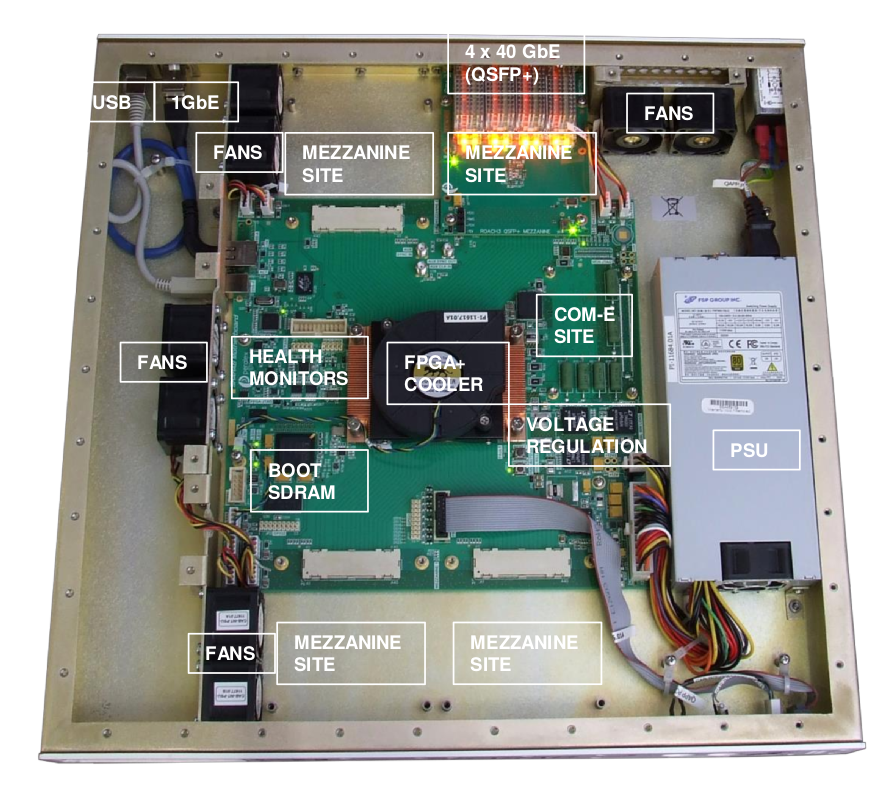
\includegraphics[height=2.7in]{skarab_hw}
  \caption{The SKARAB platform is a modular processing platform based around a Xilinx Virtex 7 FPGA with expandible mezzanine slots for memory and Ethernet ports.}
  \label{fig:skarab_hw}
\end{subfigure}%
~
\begin{subfigure}[t]{0.5\textwidth}
  \centering
  \includegraphics[height=2.7in]{snap-annotated-crop.pdf}
  \caption{The SNAP platform, developed for the HERA array, is a low-cost platform based around a Xilinx Kintex-7 FPGA. It features on-board ADCs and target applications requiring digitization, channelization and packetization of RF signals.}
  \label{fig:snap_hw}
\end{subfigure}
\caption{The latest two CASPER-supported boards. The SKARAB (a) and SNAP (b).}
\label{fig:test}
\end{figure*}

\paragraph*{SNAP}
The Smart Network ADC Processor (SNAP\footnote{\url{https://casper.berkeley.edu/wiki/SNAP}}, Figure~\ref{fig:snap_hw}) is a lightweight next generation
FPGA platform designed primarily to perform digitization, channelization and packetization of analog signal in the Hydrogen Epoch of
Reionization Array (HERA) experiment \citep{2016arXiv160607473D}. HERA requires digitization of around 700 signals at rates of 500~MS/s. In order to reduce cost and increase reliability, unlike previous CASPER platforms, the SNAP board features three onboard HMCAD1511 digitizer chips as well as an integrated synthesizer. Support for a single ZDOK interface is maintained to ensure compatibility with existing CASPER ADC daughter cards.
As with other CASPER platforms, the SNAP board is designed to be used with the 10~Gb Ethernet protocol and features two SFP+ outputs. Though lacking features of the ROACH series, such as off-chip memory and on-board CPU, the SNAP represents a flexible platform on which to implement generic RF to Ethernet digitization schemes.
The SNAP board will implement the same Microblaze-based control system as SKARAB. A CPU can also be added to the board using a simple 40-pin ribbon connector. The SNAP platform provides an interface designed to be compatible with the popular and widely available Raspberry Pi single board computer\footnote{\url{https://www.raspberrypi.org/}} which enables the SNAP to be used with software originally designed to target ROACH platforms.
% Though only recently made available to the community at large, the SNAP board 
% 
% two 10 Gbit Ethernet, and the FPGA on SNAP (the Kintex
% XC7K160T-2FFG676C chip) uses low power consumption, making the SNAP board useful
% for larger arrays. SNAP is a low-cost board. The SNAP board has one ZDOK
% connector enabling the use of the ADC cards listed below, and SNAP's onboard
% ADC's have the same specifications as the ADC16x250-8. The FPGA on the SNAP can
% be clocked either with an external frequency oscillator or with the TI LMX2581
% frequency synthesizer onboard the SNAP. The SNAP board comes with a 40-pin
% ribbon connector to interface with a  Raspberry Pi or similar computer. The
% interface to the Raspberry Pi enables the SNAP board to easily be used as a
% standalone spectrometer. FPGA gateware for the SNAP is developed using the
% JASPER tool-flow. The SNAP hardware is presented in Figure~\ref{fig:snap_hw}.


\section{CASPER Software} \label{sec:Software}
Key to the CASPER infrastructure is the ability to easily monitor and control FPGA-boards via stable, extensible, software libraries. Since the release of the first ROACH board CASPER users have been able to utilise support for the Karoo Array Telescope Control Protocol (KATCP\footnote{\url{https://casper.berkeley.edu/wiki/KATCP}}) to fill this need. KATCP is a simple text-based protocol, which now has a suite of available client libraries supporting C Lanuage\footnote{\url{https://github.com/ska-sa/katcp_devel}}, Python\footnote{\url{https://pypi.python.org/pypi/katcp}}, Ruby\footnote{\url{http://rb-katcp.rubyforge.org/}}, and LabView\footnote{\url{ftp://ftp.cv.nrao.edu/NRAO-staff/jcastro/CASPER/LabVIEW/}}.

\subsection{The CASPER Tool Flow}

Central to CASPER's wide adoption in the radio-astronomy community is the provision of a graphical toolflow which provides ``One-Click'' compile capability. Once a user has developed a design in MATLAB's Simulink environment, a single command will generate a programming file ready to be loaded onto a CASPER board. This programming file encapsulates not only the FPGA bitstream, but also meta-data about software-controllable blocks in a user's design. Coupled with the software infrastructure provided by CASPER, this allows users to load a firmware design and interact with it in real-time in an extremely straightforward and intuitive manner.
The CASPER toolflow allows users to design DSP systems without being responsible for low-level implementation details, such as ADC interfaces, or Ethernet implementations, which are handled automatically by the environment. The user is also spared the task of configuring physical design constraints such as timing requirments and FPGA pin locations, which are automatically generated based on the contents of a user's design and their target platform.
The original CASPER toolflow was inherited from the Berkeley Wireless Research Center's BEE2 project\footnote{\url{http://bee2.eecs.berkeley.edu/wiki/BEE2wiki.html}} which created the ``bee\_xps'' flow. This was based around a MATLAB object oriented framework for generating a Xilinx Embedded Development Kit (EDK) project, along with associated constraints, and compiling it into a \emph{.bof} file -- a container for the bitstream and its meta-data.
The bee\_xps flow served the CASPER community well, but had a number of drawbacks:
\begin{enumerate}
 \item Few members of the CASPER community were familiar with MATLAB Object Oriented Programming, creating an immediate barrier to users becoming toolflow developers.
 \item The bee\_xps flow is entirely reliant on MATLAB. This goes against the desires of the CASPER community for a free, open-source flow. Where aspects of the flow could in-principle be reimplemented outside of MATLAB, the monolithic nature of the bee\_xps flow made this difficult.
 \item The bee\_xps flow is strongly coupled to MATLAB's Simulink design entry tool. While this is an advantage for new users, who appreciate a graphical interface, advanced users and developers have long been requesting alternative design input methods.
 \item the bee\_xps flow uses a Xilinx's ISE package, which has not been updated since 2013 and is not supported by the latest generations of Xilinx FPGAs.
\end{enumerate}

The last of these drawbacks became particularly significant with the release of the SKARAB and SNAP hardware platforms, which are the last generation of FPGAs to support ISE. This has led to the development of a new toolflow, nominally under the name \emph{JASPER}, designed to support the latest generations of FPGAs and alleviate some of the shortcomings of bee\_xps.
The JASPER flow has the following features:
\begin{enumerate}
 \item Written in pure Python 2.7, with minimal dependencies.
 \item Supports the same Simulink design entry method used by bee\_xps, allowing portability of existing designs to the new flow.
 \item Designed to be modular, with the design entry method de-coupled from the management of contstraints and interface code which the toolflow aims to hide from the designer.
 \item The flow is also decoupled from the FPGA vendor's compilation tools. This allows the JASPER flow to support both Xilinx ISE (required by older platforms) as well as Xilinx's new Vivado software suite required by the newest generation of FPGAs.
\end{enumerate}

...Put something here to connect to what Adam wrote below...


%% Jack Hickish to introduce this and explain history

%% Adam Isaacson to explain the latest additions
% The JASPER tool flow is currently being upgraded to make provision for additional front ends and back ends besides Simulink and Xilinx, respectively. This will prevent the developer from being tied down to a specific software package and FPGA platform \cite{Isaac16}. The current upgrades are presented in Figure~\ref{fig:jasper_ug_bd} \cite{Isaac16}.

% \begin{figure}[h]
% \centering
% 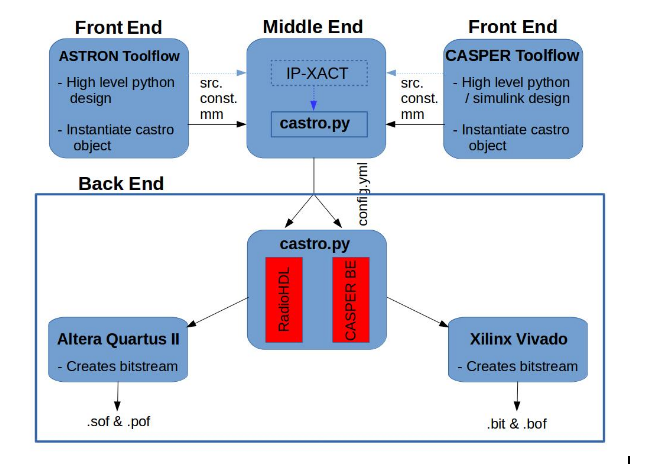
\includegraphics[width=150mm, scale=0.5]{jasper_ug_bd}
% \caption{JASPER Upgrade Tool Flow Diagram}
% \label{fig:jasper_ug_bd}
% \end{figure}

The Front-End includes the structural VHDL or any modelling tools e.g. Matlab/Simulink, Labview, Sci-Lab/Sci-Cos and MyHDL. It includes a script which will instantiate the python classes inside the Middle End process \cite{Isaac16}.

The python classes are located in the Middle End (castro.py) file. In the future, it is likely that the Front End will come in through another interface e.g. possibly IP-XACT in order to make provision to interface to other simulation tools e.g. Sci-Cos and Sci-Lab. This interface is denoted by the dashed lines in Figure~\ref{fig:jasper_ug_bd}. IP-XACT is an IEEE standard and is used to integrate different IP packages together, provided that the IP interfacing meets the IP-XACT standard. The IP-XACT interface would be in the form of an XML script. The decision to utilise IP-XACT has not been finalised yet. The castro.py is passed all the Front End memory map, constraints and source files. The castro.py script takes this metadata from the Front End and dumps all of this metadata into a YAML configuration file (config.yml). It should be noted that the Middle End module is not platform agnostic due to the hardware and platform metadata \cite{Isaac16}.

The Back End consists of the same castro python class that exists in the Middle End. The castro.py python script will load the config.yml file/metadata and instantiate python objects with this metadata, which will either be sent to RadioHDL if targeting the Altera hardware or the Casper Back End, if targeting the Xilinx hardware. This will also allow the user to target other vendor hardware in the future e.g. Lattice and Actel and due to the common castro.py python script, it will easier to just add an additional back end \cite{Isaac16}.

The RadioHDL process will then generate the necessary Quartus project files and run the compiler. The output of the process will be the Altera FPGA SRAM Object file (sof) and Programming Object File (pof). The Casper Back End generates the necessary tcl scripts, which runs the Vivado compiler. The output of the process is the Xilinx FPGA bit and Borph Object File (bof) programmable files \cite{Isaac16}.

The current release of the JASPER tool flow actually includes the castro python class and the CASPER back end makes provision for both Xilinx ISE and Vivado. The JASPER tool flow also makes provision for the SKARAB platform and the generation of the fpg configuration files, which are used for the ROACH2 and SKARAB configuration \cite{Balla16}.

%% Adam Isaacson / Jack Hickish

\subsection{CASPER DSP Libraries}

%% Andrew Martens + anyone else keen to contribute

% NOTE: First draft of section, please feel free to edit (Griffin)
% TODO: add CBASS-south, AVN Ghana, KuPol to instrument list

In order to quickly and easily develop new radio astronomy instruments a number
of DSP blocks have been developed for use in CASPER board firmware. Typical
instruments such as spectrometers, beamformers, correlators, ADC recorders, and
DAC signal generators are constructed from this library of DSP blocks.

These blocks are based on the low-level logical units provided by the Xilinx
Simulink library and the generic Simulink libraries. Configurable low-level DSP
blocks are then used to build more complex, high-level DSP blocks. This
heirarchical design style enables quick and uniform logic development through
block reuse. High-level blocks include configuration parameters which are
propagated through the low-level logic to update the underlying logic. Thus,
generic blocks such as streaming FFTs and vector accumulators are included in
the library, and configured when placed into a firmware design.

Matlab Simulink provides a 2-D, heirarchical design and simulation environment
useful for firmware design. Individual DSP blocks are placed into a model
design, and connected via data lines. Once a firmware model has been laid out
test vectors can be simulated through the system to verify the logic with a test
bench.

Xilinx provides the basic libraries to build firmware for their FPGAs. Basic
blocks include logic gates, multipliers, adders, signal delays, FIFO buffers and
block RAM (BRAM) interfaces. Blocks in the CASPER library are written using
these basis blocks. Blocks can also be wrappers for HDL code, such as with the
external interfaces. A number of specialized basic blocks have been written in
the CASPER library for radio astronomy applications. For example, many low-bit
complex multipliers are often used in correlation, to improve the resource
efficiency a specialized 4-bit multiplier has been written. Also typical in
firmware design is signal reorders and transposes, general blocks have been
written to facilitate ease of BRAM memory use for these operations.
Documentation on the CASPER library can be found
online\footnote{https://casper.berkeley.edu/wiki/Block\_Documentation}.

Using these basic logic and memory building blocks more complex DSP modules have
been developed. At the core of many radio astronomy instruments is a fast Fourier
Transform operation. A generic FFT module is implemented using a radix-2,
biplex, decimation-in-time design. This module computes the Fourier Transform on
a window of $2^N$ complex samples and is highly configurable. An efficient
real-input FFT and a multi-input 'wideband' FFT module have been implemented
using the generic FFT. In order reduce FFT sidelobe leakage due to the finite
window size an FIR module has been implemented to work in unison with the FFT to
create a poly-phase filterbank (PFB), see \S 4.2 of \citet{price13}.

Working with signals in time and frequency domain often requires large data
reorderings. A common operation is to perform a corner turn, i.e. a matrix
transpose on a window of data. For small windows this is done in BRAM, but
larger corner turns are done via external memory, such as the QDR, or with the
network architecture. Blocks for more complex data reorders such as interleaving
have also been implemented.

Modules for the cross-correlation operation in an FX correlator have ben
implemented in the library. A complex multiply and accumulate (CMAC) block for
small correlators, usually on a single board for a small number of inputs, can
be used in a matrix-style design. For large-N correlator systems distributed
across multiple boards a streaming windowed x-engine can be used, see \S 3.2 and
3.3 of \citet{hickish14}.

A number of vector accumulators modules are in the library.
Small vectors, such as those from a spectrometer, are implemented in BRAM. While
large vectors, such as the cross-correlations of a correlator are implemented
with QDR or DRAM memory. These accumulators include an interface to be accessed
via software during runtime.

Blocks for including dynamic delays in beamformer and correlator systems have
been implemented. A configurable 'coarse' delay can be applied before the FFT
operation, while a 'fine' delay can be applied post-FFT with a phase correction.
These delays can be combined with a software interface to act as a fringe
tracking module.

Similarly to the fine delay module a gain equalizer module is implemented to
dynamically update complex gain coefficients which are applied post-FFT. This is
often used in unison with a 4-bit quantizer block to reduce the signal bitwidth
before correlation.

In addition to the generic DSP blocks a number of external interfaces known as
'yellow blocks' have been designed to interface with external hardware such as
ADCs, DACs, software interface registers, QDR  and DRAM memory, and network
interfaces. Each yellow block has been developed for a specific external module.
With in the Simulink environment a yellow block acts as a place holder for an
external interface. During the synthesis toolflow the appropriate HDL for the
external module is included into the design.

The main collaboration library is hosted on
github\footnote{github.com/casper-astro/mlib\_devel}, SKA South Africa
is one of the main contributors to the library and similarly host their own
version\footnote{github.com/ska-sa/mlib\_devel} on github. A number of
other project and institutional forks exist, features from these repositories
are regularly merged into the main library.



\section{CASPER Deployments} \label{sec:Deployments}

Tables \ref{table:casper-instruments-spectrometers}, \ref{table:casper-instruments-mkid} and \ref{table:casper-instruments-correlators} list, respectively, spectrometers, MKID readouts, and correlators/beamformers built on CASPER technologies.
These instruments include those delivering groundbreaking science such as the Event Horizon Telescope \citep{Johnson1242}, ..., ...

\begin{longtable}{ccp{10cm}}
  Instrument & Year & Description \\
  \hline
  Leuschner Spectrometer & 2015 & Dual-polarization, 12 MHz, 8192 channel spectrometer for UC Berkeley's Leuschner Radio Observatory. Based on ROACH1 and ADC2x1000-8\footnote{\url{https://github.com/domagalski/leuschner-spectrometer}} \\
  DSN Transient Observatory & 2016 & Versatile signal processor for commensal astronomy during DSN data downlinks, featuring Kurtosis Spectrometer and pulse detection. Based on a pair of ROACH boards with KATADCs \citep{dsn-transient-observatory} \\
  RATTY            & 2012 & Transient / RFI Monitor for SKA-SA site monitoring implemented on a single ROACH board \citep{Foley01082016, Manley thesis}. \\
  cycSpec          & 2012 & Real-time cyclic spectrometer, deployed at Arecibo (ROACH) and GBT (ROACH2) on consecutive generations of hardware. Implements a filterbank of 128~MHz overlapping channels used to feed GPU processors \citep{Jones et al (in prep)}. \\
  GRASP            & 2016 & 100 MHz bandwidth full-stokes spectrometer for the Gauribidnaur Radio Solar spectro-Polarimter. Implemented on a single ROACH board with quADC digitizer \citep{Indrajit}. \\
  HIPSR            & 2014 & 400~MHz bandwidth 8192 channel spectrometer and high time-resolution system for the Parkes multibeam receiver. Based on 13 ROACH1 boards and 13 ADC2x1000-8 digitizers\footnote{\url{http://telegraphic.github.io/hipsr/overview.html}}. \\
  Skynet           & 2012 & Single board ROACH-based educational spectrometer for the Green Bank 20m telescope. Provides 500MHz BW, dual-polarized input, and 1024 channels \citep{skynet}. \\
  GBTrans          & 2014 & Single board ROACH-based transient event spectrometer for the Green Bank 20m telescope, 500MHz BW, dual-polarized input, and 2048 channels \citep{gbtrans}. \\
  KuPol            & 2014 & 6 GHz bandwidth full Stokes spectrometer, implemented with 12 ROACH boards and 24 ADC2x1000-8 digitizers \citep{2013arXiv1303.2131M}. \\
  Canberra DSN     & 2016 & 16~GHz single pol or 8~GHz dual-pol spectrometer. Implemented using 4 ROACH2 boards \citep{Kocz, in prep}. \\
  BPSR             & 2009 & 400~MHz bandwidth, 13-beam fast-dump spectrometer for the Parkes multibeam receiver. Originally implemented with iBOBs. Upgraded in 2012 to use 13 ROACH boards \citep{2010MNRAS.409..619K}. \\
  NUPPI            & 2011 & 512~MHz digitization and flexible (32-1024 channel) channeliser for pulsar observations. Implemented using a single ROACH board with ADC2x1000-8 digitizer \citep{2014MNRAS.443.3752L}. \\
  VEGAS            & 2014 & Versatile spectrometer for the GBT, providing up to 10GHz BW for 1 dual-polarized input or 1.25GHz BW for 8x dual-polarized inputs. Features wideband modes and narrowband modes with 8 digitally tuned sub-bands within the 1.25GHz BW. Implemented using 8 ROACH2 boards with ADC1x5000-8 digitizers \citep{chennamangalam2014gpu}. \\
  GAVRT            & 2009-2012 & 8~GHz instantaneous bandwidth transient capture buffer with real-time incoherent dedispersion trigger. Implemented with 8 iBOBs, 16 ADC2x1000-8s and a BEE2 \citep{jon10, JonesDSS28}. \\
  ALMA Phased Array& 2014 & 8 ROACH2 system for time-tagging, ethernet packetization and VDIF (VLBI) formatting \citep{2012evn..confE..53A}. \\
  GUPPI            & 2009 & Pulsar processor with the Green Bank Telescope. Provides full stokes polarimetry and ethernet packetizing with up to 800 MHz BW. Based on a pair of iBOB boards with ADC2x1000-8 digitizers and a BEE2 \citep{guppi}. \\
  CASPSR           & 2009 & 400~MHz bandwith packetizer for GPU-based pulsar processing backend at the Parkes telescope. Originally implemented with an iBOB. Later upgraded to a ROACH board with ADC2x1000-8 digitizer\footnote{\url{https://astronomy.swin.edu.au/pulsar/?topic=caspsr}} \\
  Fly's Eye        & 2007 & High time-resolution spectrometer for the 42-dish Allen Telescope Array. Based on 11 iBOB boards with 22 ADC2x1000-8 digitizers \citep{flyseye} \\
  SERENDIP        & 2009+ & 200~MHz spectrometer with 1.5~Hz resolution, fed from the Arecibo L-band Feed Array. SERENDIP V.v was deployed in 2009 \citep{seti} and was implemented with an iBOB and BEE2. The latest generation, SERENDIP VI, uses a single ROACH2 and ADC1x5000-8 digitizer to process >1~GHz bandwidth. SERENDIP VI has been deployed at both the Green Bank and Arecibo Observatories. \\
  \caption{Spectrometers and packetizers powered by CASPER hardware.}
  \label{table:casper-instruments-spectrometers}
\end{longtable}


\begin{longtable}{ccp{10cm}}
  Instrument & Year & Description \\
  \hline
  BLAST-TNG        & 2017 &  2.5~m Balloon-Borne Submillimeter Polarimeter with CASPER MKID readout system. BAsed on 5 ROACH2 boards with MUSIC-DAC/ADC cards \citep{galitzki2014balloon}. \\
  HOLMES           & 2018 & Electron Neutrino Mass measurement experiment with CASPER-based microwave SQUID readout system, based on 35 ROACH2 boards with MUSIC-ADC/DAC cards \cite{Alpert2015, Ferri2016179.} \\
  Columbia MKID    & 2012 & ROACH (later ROACH2) based MKID readout system with CASPER-based tone generation, digitization and coarse channelization. Feeds non-CASPER HPC processors \citep{mccarrick_2014}. \\
  Mustang2         & 2015 & 90GHz FPA TES bolometer array, with Microwave-multiplexed SQUIDs. Based on 4 ROACH boards \citep{2016JLTP..184..460S, 2014JLTP..176..808D}.  \\
  COMAP            & Development & 4~GHz, 19-pixel MKID readout system, implemented using 38 ROACH2 boards \footnote{\url{http://www.astro.caltech.edu/CRAL/projects.html}}. \\
  ARCONS           & 2011 & 250-pixel MKID readout system with 500~MHz bandwidth between 3.5-5.5~GHz. Implemented using 8 ROACH boards with MUSIC ADC/DAC cards \citep{10.1086/674013}. \\
  DARKNESS         & 2016 & 10,000 MKID pixel readout system with 2~GHz bandwidth between 4-8~GHz. Implemented with 10 ROACH2 boards and custom ADC/DAC/IF cards \citep{in prep}. \\
  MEC              & 2017 & Expansion of DARKNESS system to accommodate 20,000 pixel readout, using 20 ROACH2 boards with custom ADC/DAC/IF cards \citep{in prep}. \\
  \caption{MKID readout systems powered by CASPER hardware.}
  \label{table:casper-instruments-mkid}
\end{longtable}

\begin{longtable}{ccp{10cm}}
  Instrument & Year & Description \\
  \hline
  ARI              & 2012 & 21-cm dual-antenna interferometer for teaching purposes. Based on a single ROACH and ADC2x1000-8 \citep{MScSalas2014}. \\
  pocketcorr       & 2014 &  Multi-platform (ROACH, ROACH2, SNAP) single-board FX correlator. Used in HYPERION deployment and PAPER testing\footnote{\url{https://github.com/domagalski/pocketcorr}} \\
  MeerKAT          & Development & ``Facility Instrument'' capable of producing various data products over 856~MHz bandwidth. Modes include 32k channel, 64 dual-pol antenna correlator, beamformer and transient buffer. Currently based on ROACH2 boards, with a SKARAB upgrade forthcoming \citep{MeerKAT CBF Requirement Spec}. \\
  MeerKAT AR-1     & 2016 & MeetKAT Array Release 1. Beamformer and correlator system operating between 900 and 1670 MHz with a digital bandwidth of 856 MHz\footnote{\url{http://public.ska.ac.za/meerkat/meerkat-schedule}} \\
  KAT7             & 2010 & 7 dual-pol antenna full-stokes FX correlator, based on 16 ROACH boards \cite{Foley01082016}, Manley thesis \\
  AMI              & 2015 & 5~GHz, 4096 channel FX Correlator for the 10-antenna and 8-antenna Arcminute Microkelvin Imager arrays. Based on 18 ROACH2 boards with 36 ADC1x5000-8 digitizers \citep{Zwart21122008,Hickish et al. (in prep)}. \\
  %SWARM Correlator & & & & \\
  Medicina FFTT    & 2014 & A digitization, channelisation, beamforming and correlation system, used to demonstrate direct-imaging on the BEST-2 Array. Based on 3 ROACH1 boards and an ADC64x64-12 diitizer \citep{Foster11042014}. \\
  MITEoR           & 2014 & 50~MHz bandwidth, 64 dual-polarization antenna FX correlator, used to investigate spatial-FFT correlation methods. Implemented using 4 ROACH2 boards each with ADC64x64-12 digitizers \citep{2014MNRAS.445.1084Z}. \\
  FLAG             & 2016 & 19 dual-polarized input PAF system for the GBT. Provides 150 MHz BW using 5 ROACH2 boards \citep{gb_flag, gb_beamformer}. \\
  BIRALES          & 2016 & 14~MHz bandwidth, 32-input digitization and channelisation system for software beamformer. Implemented using a single ROACH board with ADC64x64-12 digitizer \citep{7180719}. \\
  Starburst        & 2016 & 5 GHz, single-baseline FX correlator, based on 4 ROACH2 boards with 8 ADC1x5000-8 digitizers \citep{Monroe, private comm}. \\
  MAD              & 2013 & 16~MHz, 18-input FX correlator and beamforming system for low-frequency array prototyping for the SKA. Implemented using a single ROACH board with ADC64x64-12 digitizer \citep{Pupillo2015, RDS:RDS20336}. \\
  PAPER            & 2010 & 100~MHz FX correlator originally based on iBOBs, and later upgraded to ROACH, and then ROACH2 boards. Current correlator has 256 inputs, and is based on a CASPER `F' stage using 8 ROACH2 boards followed by a GPU-based `X' stage \citep{2010AJ....139.1468P, 2014ApJ...788..106P, 2015ApJ...809...61A}. \\
  HERA             & Development & 100~MHz bandwidth, 700-input FX correlator, constructed using $O(100)$ SNAP boards for digitization and channelization. `X' stage will be carried out either on GPU- or FPGA-based platforms, depending on availability and cost \citep{2016arXiv160607473D}. \\
  AMiBA            & 2016 & Upgrade of the AmiBA wideband analog correlator. 7 dual-pol antenna 4.48~GHz bandwidth FX correlator, implemented on 7 ROACH2 boards with 14 ADC1x5000-8 digitizers \citep{amiba-adc, amiba-interim}. \\
  LEDA             & 2012 & 58~MHz 512-input digitization, channelization and packetization system for a GPU correlator backend. Implemented using 16 ROACH2 boards with 32 ADC16x250-8 digitizers \citep{doi:10.1142/S2251171715500038}.\\
  \caption{Correlators and beamformers using CASPER hardware for either their `F', `X' or beamforming stages.}
  \label{table:casper-instruments-correlators}
\end{longtable}


\section{Future Directions \& Challenges} \label{sec:Future}


\section{Conclusions} \label{sec:Conclusions}
Over the past decade, ...With over 500 CASPER FPGA-boards delivered to collaborators, and more than 50 instruments 

\bibliographystyle{ws-jai}

\bibliography{casper-2016}


\end{document}
